% !TEX root = ../main.tex

\subsection{Project II - Circle Game}
\label{sec:impl:project:ii}

\newcommand{\gi}{\textbf{CG1}}
\newcommand{\gii}{\textbf{CG2}}
\newcommand{\giii}{\textbf{CG3}}
\newcommand{\giv}{\textbf{CG4}}

This section describes the implementation of a game that was developed for the {\DK}.
The game is simple, but \gls{cpu} intensive, and was developed as a part of measuring the performance of {\rust} on the {\gecko}.
% The results gathered from the measurements are presented and discussed in \autoref{chap:results}.

\subsubsection{Goal}

The {\cg} application was developed to compare the performance between {\rust} and {\C}.
It is not easy to give a performance metric, and compare two languages directly against each other based on only one application like this.
However, an application like this gives us a good indication of whether the two languages differ or have roughly the same performance.

\subsubsection{Requirements}

The requirements that were made for the game are summarized in \autoref{tab:project:ii:requirements}.
{\gi} and {\gii} sets the hardware requirements for the application; we chose to restrict it to the {\DK} because of its on-board \gls{lcd} screen and header pins.
The two modes mentioned in {\giii} was deemed necessary for testing purposes and for measuring performance, respectively.
{\giv} specifies the performance metric, \gls{fps} was chosen because it is an intuitive way of measuring performance.
The result will be a number that represents how many iterations of the game's main loop have been executed each second.

\begin{table}[H]
  \centering
  \begin{tabular}{c|p{8cm}}
    \textbf{Requirement} & \textbf{Description} \\
    \hline
     \gi & The game should be made for the {\DK}. \\
     \gii & The graphics should be rendered on the \gls{lcd} screen. \\
     \giii & The game should support two modes, it should be controlled with a gamepad, or be self-playable. \\
     \giv & The performance should be measured in the number of \gls{fps}. \\
    \hline
  \end{tabular}

  \caption{Requirements for the {\cg}}
  \label{tab:project:ii:requirements}
\end{table}

\subsubsection{Description}

The game was first written in {\C} by one of our supervisors as part of the TDT4258 \footnote{\url{http://www.ntnu.edu/studies/courses/TDT4258}} course at NTNU, and later ported by us to {\rust}.
It is a simple game that consists of three components that are drawn to the screen; two circles and an obstacle.
The two circles can be controlled with a gamepad that is connected to the {\DK}'s header pins, \autoref{fig:circle_game} shows a setup of the game.
The obstacle is randomly generated and has either one or two gaps, it spawns on top of the screen and is moved down one step for every iteration of the game loop.
The goal of the game is to avoid any collision between the circles and the obstacle.
If the obstacle reaches the bottom of the screen without colliding with any of the circles the game score is increased.
However, if any of the circles collide with the obstacle, the game is over, and the score is reset to 0.

\begin{figure}[ht]
  \centering
  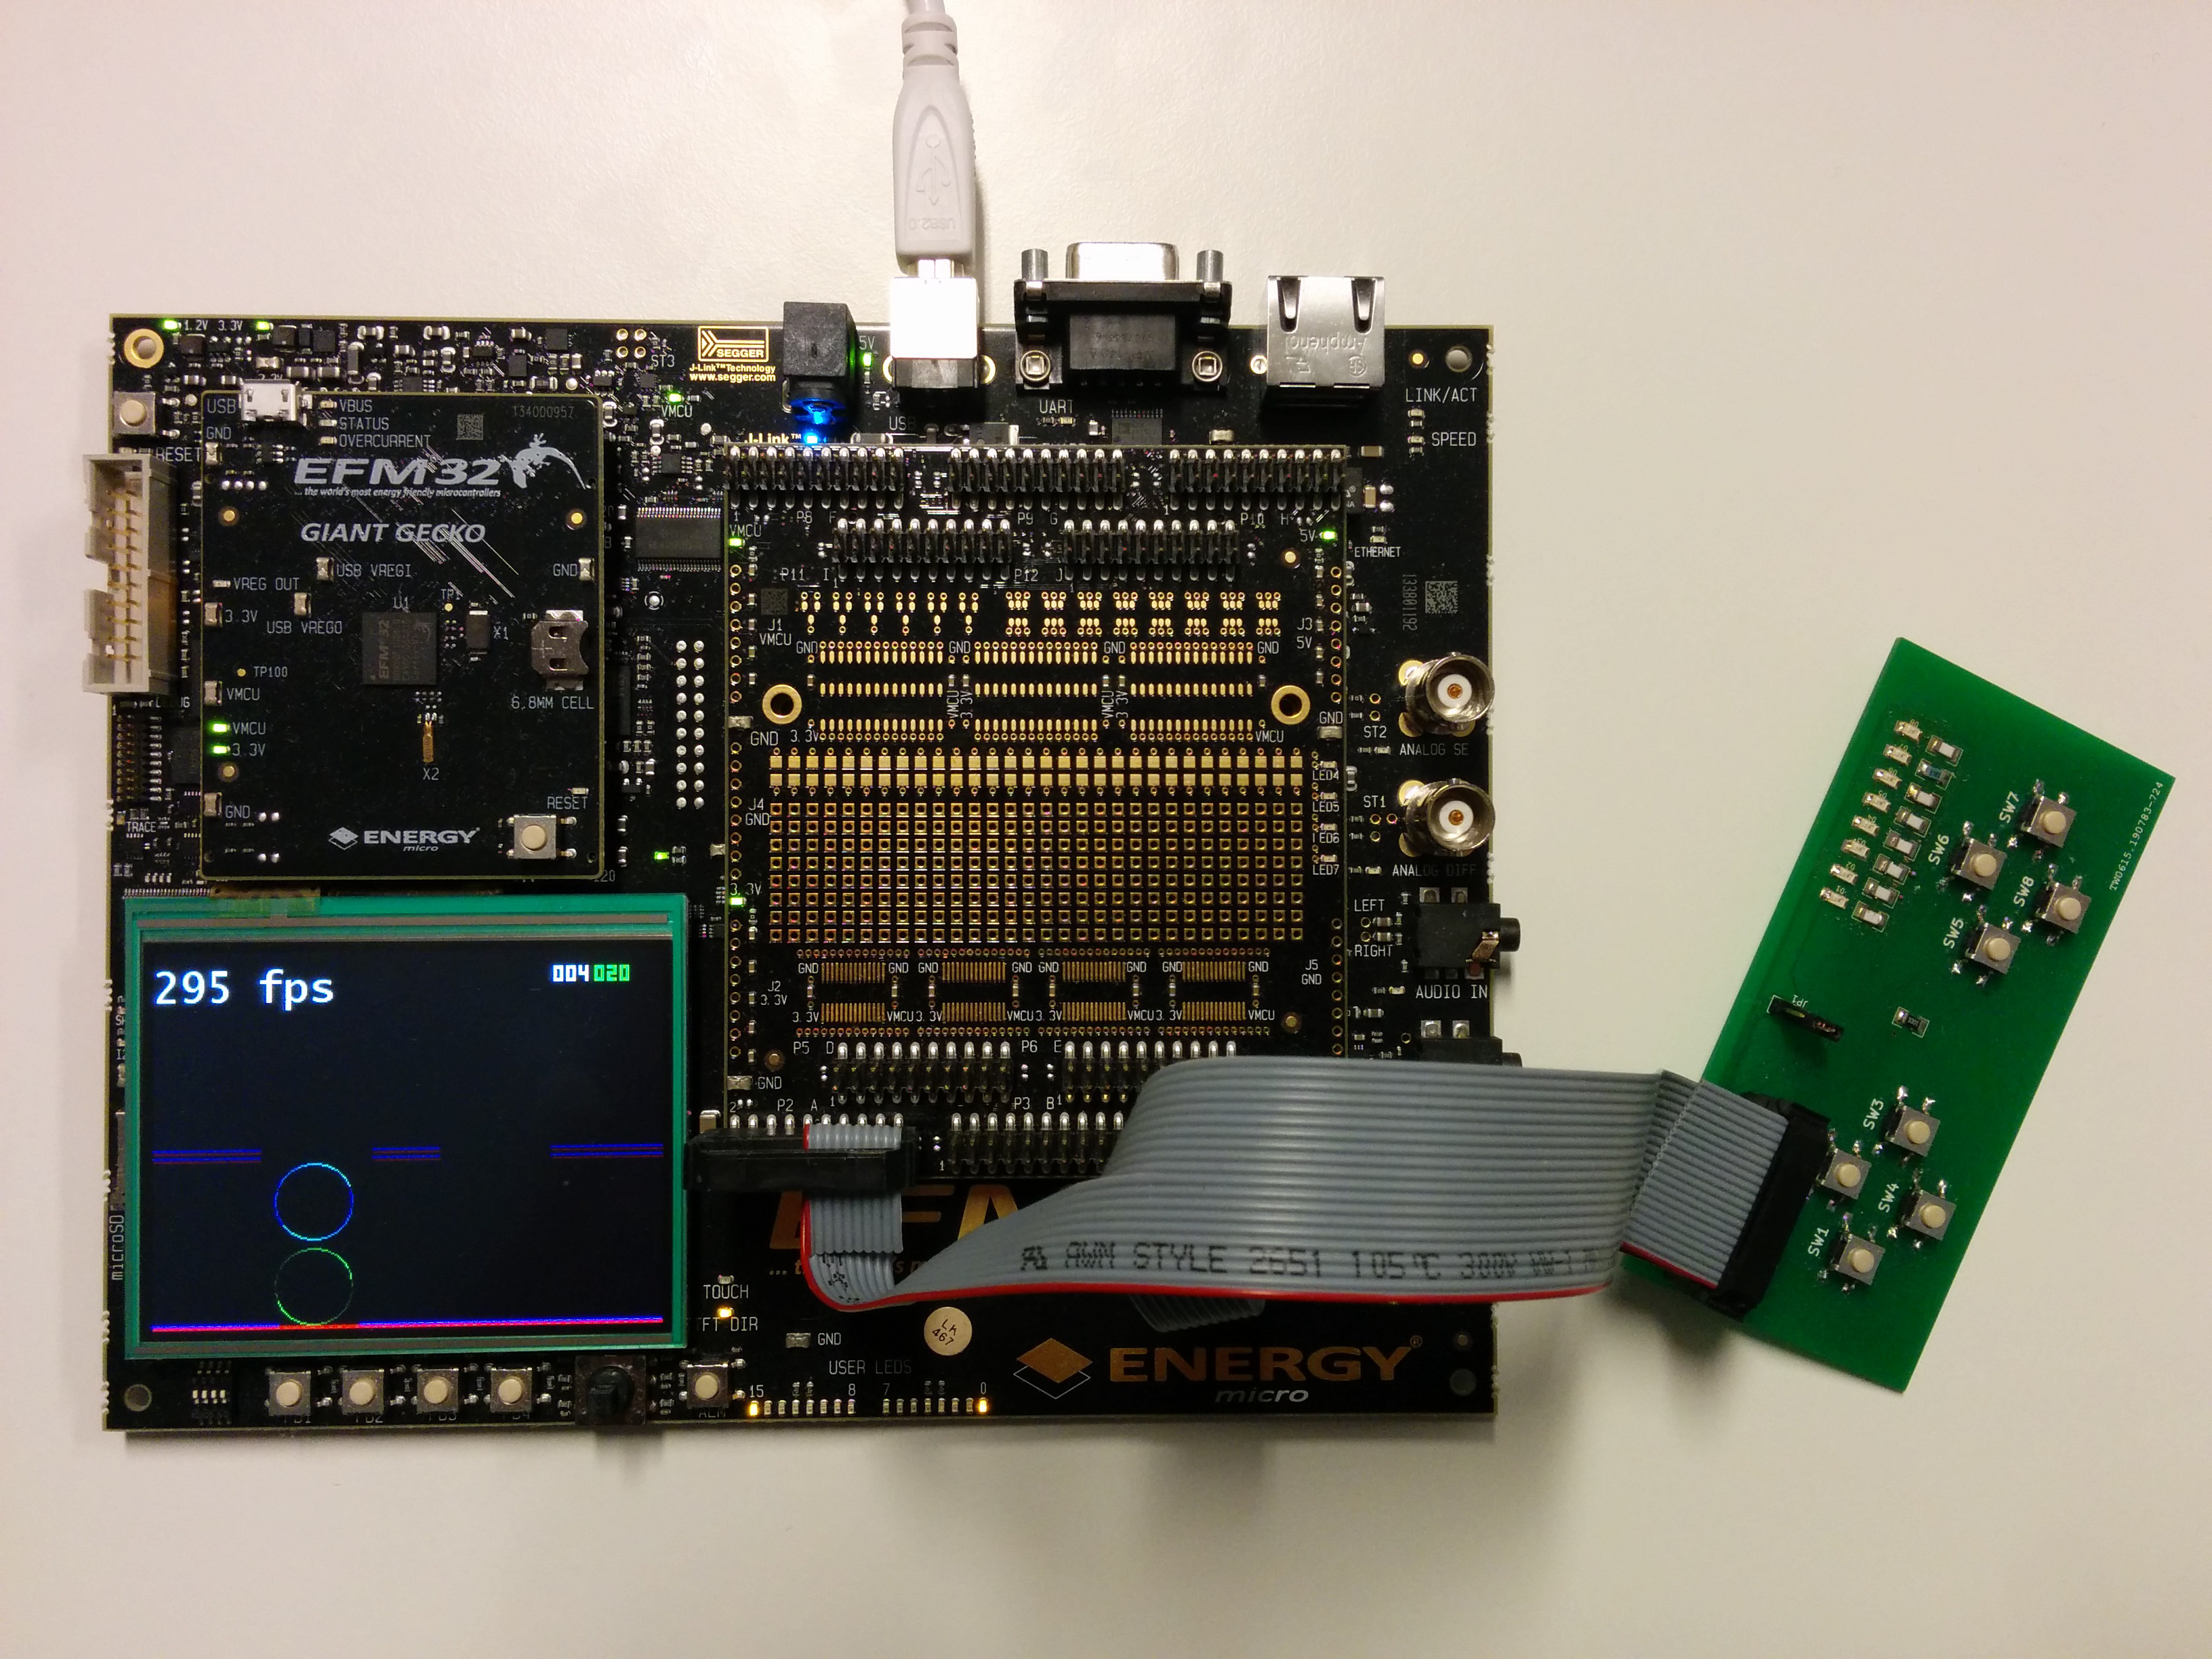
\includegraphics[width=0.5\textwidth]{figures/circle-game.jpg}
  \caption{{\cg} running on the {\DK} with the attached gamepad}
  \label{fig:circle_game}
\end{figure}

The game consists of three phases; initialization, reset, and the game loop.
Pseudo code for the game is shown in \autoref{lst:game_loop}, as the code suggest, most of the work is done in the game loop.
We calculate the \gls{fps} for the game by increasing a counter for every iteration of the loop.
An interrupt is also set up to be triggered once every second, which consecutively updates the \gls{fps} and resets the counter.

The game also has support for playing by itself.
This mode is necessary because the optimized versions of the game run with several hundreds of iterations each second, and it makes it easier to collect the results from the performance test.

\begin{listing}[ht]
  \begin{rustcode}
static mut FRAME_COUNT = 0;
static mut LAST_FRAME_COUNT = 0;

fn main() {
  init();  // Run Microcontroller initialization
  reset(); // Reset the Game Environment
  loop {   // Game Loop
    let input = get_user_input(); // Get input from user buttons
    player.move(input);           // Move Player according to input
    obstacle.move();              // Move obstacle
    // Check if collision occurred
    if check_collision(player, obstacle) {
      game_over(); // Report game is over to player
      reset();     // Reset the Game Environment
    }
    redraw_screen(); // Update contents on the LCD
    FRAME_COUNT += 1;
  }
}
// Interrupt handled once each second
extern fn SysTick_Handler() {
  LAST_FRAME_COUNT = FRAME_COUNT;
  FRAME_COUNT = 0;
}
  \end{rustcode}
  \caption{Pseudo code of the {\cg}}
  \label{lst:game_loop}
\end{listing}
